%TBD: remove results from inline text and into tables
\chapter{Upper limits}

The $\PgUc$ peak is not significantly observed in the  mass spectrum in the \PbPb data.
The significance of $\PgUc$ peak is 0.86$\,\sigma$, evaluated form the profile likelihood ratio, as shown in \fig{fig:3S-significance}. In this section we quantify the relative suppression of the 3S signal state.

\begin{figure}[hbtp]
  \begin{center}
{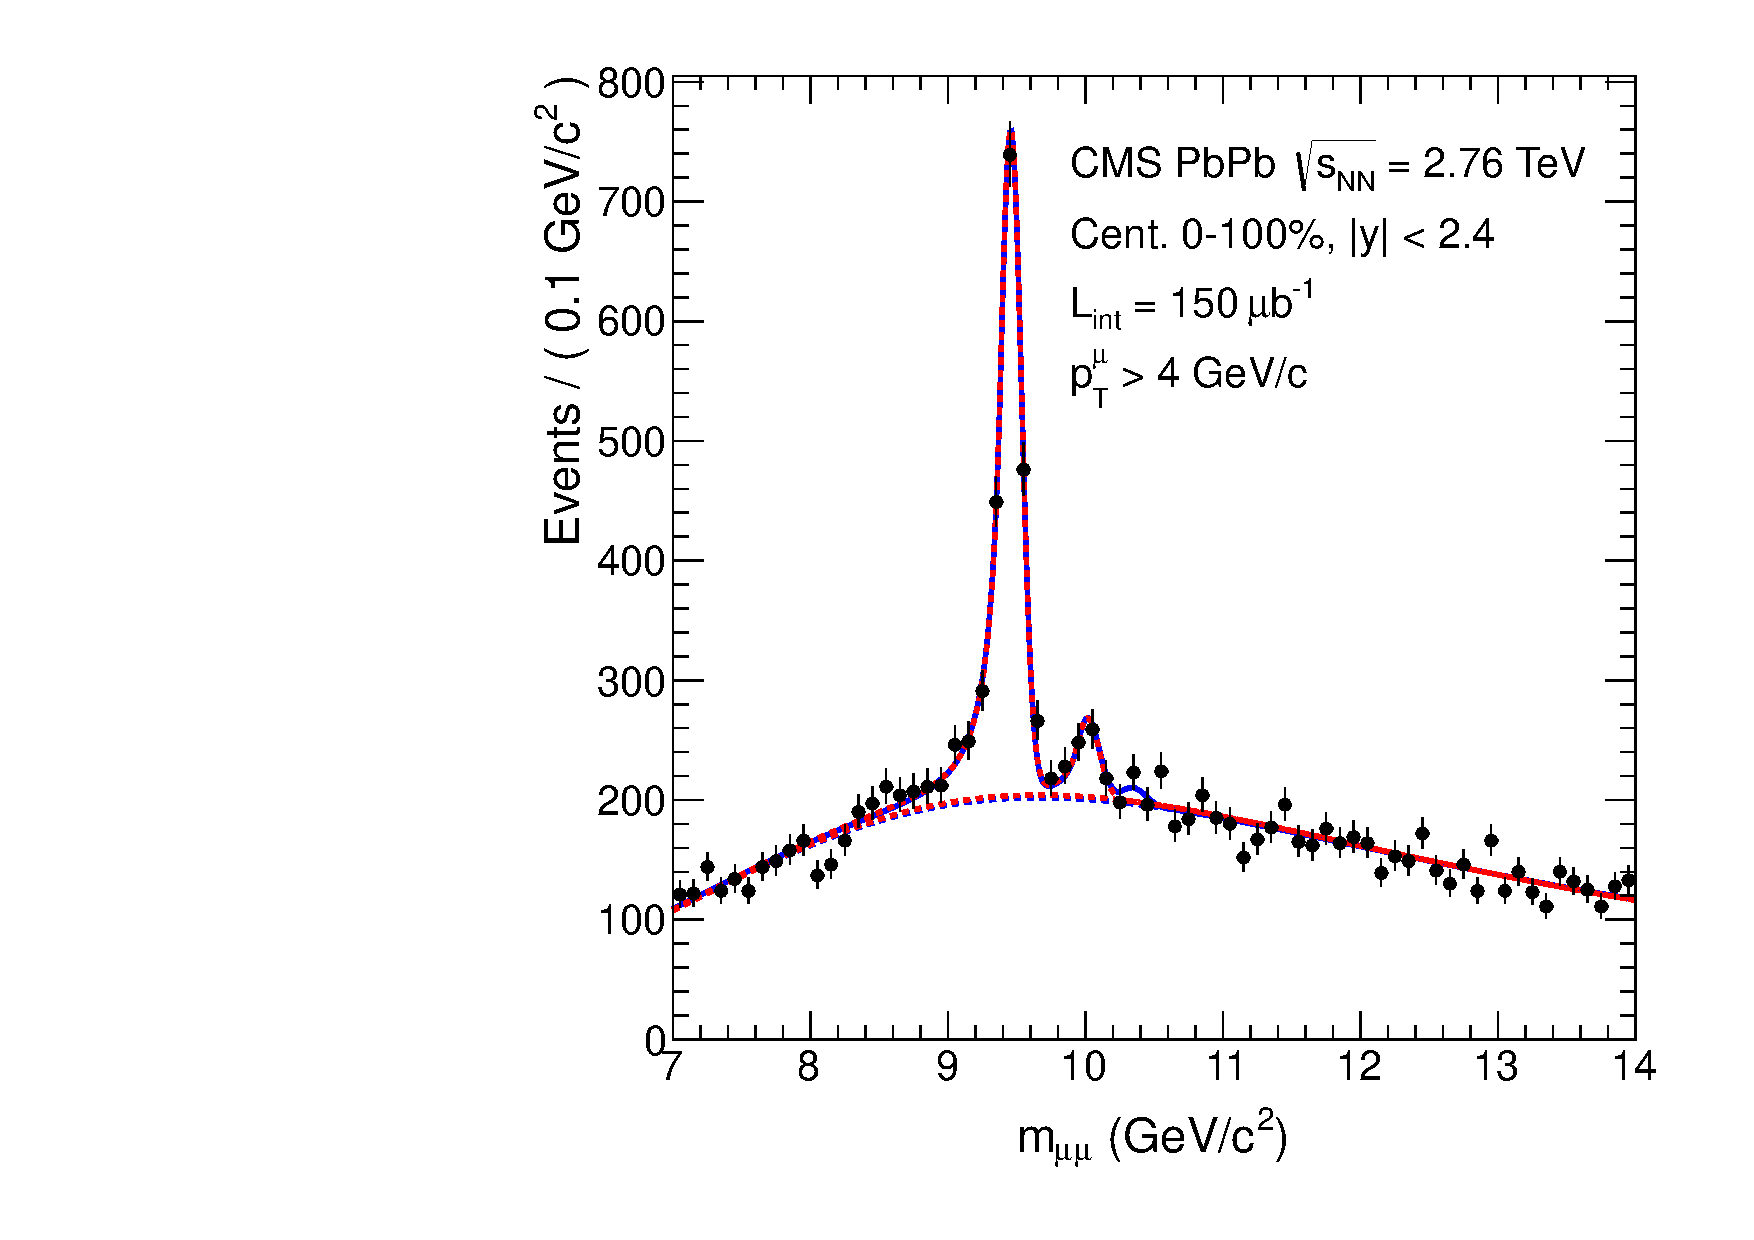
\includegraphics[angle=0,width=0.45\textwidth]{figures/limits/Y3S_significance.pdf}}
   \caption{$\PgUc$ significance, estimated via likelihood ratio, by allowing and disallowing $\PgUc$ p.d.f. in two fits.
}
    \label{fig:3S-significance}
  \end{center}
\end{figure}

%\subsection{The  Feldman-Cousins and $CL_{s}$ prescription}

In some of the centrality bins the data is affected by large downward fluctuations of the background yielding negative yields for the signal \PgUc. We proceed then to set upper limits for the signal 3S .

Approximate methods of confidence interval construction, in particular, the likelihood-ratio method, are often used in order to reduce computation. However, true confidence intervals can be obtained using the original (defining) Neyman construction~\cite{Neyman}.  
Therefore we opted for the unified Feldman-Cousins (FC) approach since this treatment solves the problem whether to set an upper limit or two-sided intervals if the choice is based on the data alone as in our case. 

 As a cross check we also present a pure frequentist approach, the \textit{modified}, or \textit{conservative} $CL_s$ criterion. Here, we use the ratio of $p$-values, $CL_{s}=CL_{sb}/CL_{b}$, instead of the numerator only, to set an upper limit on the single and double ratios involving the 3S.  Finally other implementations based on 95\% credible intervals are presented as cross-checks.

\subsubsection{Single ratio $R_{3}$ limits}
Instead on setting upper limits for the \PgUc signal per se we use the single ratio of the third peak over the first peak ($R_{3}$) in PbPb as our parameter of interest. The idea of the method can be formulated in terms of hypothesis testing in a frequentist approach.  (for an explanation see~\cite{alexread}).  
We define $H_b$ as the alternative hypothesis that no signal 3S is present over the background (single ratio of zero) and $H_{sb}$ the null hypothesis that the signal is indeed present. In order to quantify the degree in which each hypotheses
are favored or excluded by the experimental observation one chooses a
test-statistics which ranks the possible experimental outcomes. A
commonly used test statistics consist as the ratio of the likelihood
function in both hypotheses: $Q=L_{sb}/L_b$, for our study the test statistic of choice is $-2\ln Q$. 

We introduce the systematic uncertainties into the model via a nuisance parameter. Variation of such parameter corresponds to certain systematic uncertainty. The nuisance parameter is either profiled or marginalized depending on whether we are using the frequentist approach or the Bayesian one. 

The computed 95\% CL upper limit with FC is: 0.0737 +/- 0.0014.
%https://espace.cern.ch/cms-heavyion/upsilon/fitting/Upper%20Limits.aspx
Cross checks based on alternative methods are provided in Appendix~\ref{sec:app_limits}. 


\begin{figure}[hbtp]
  \begin{center}
{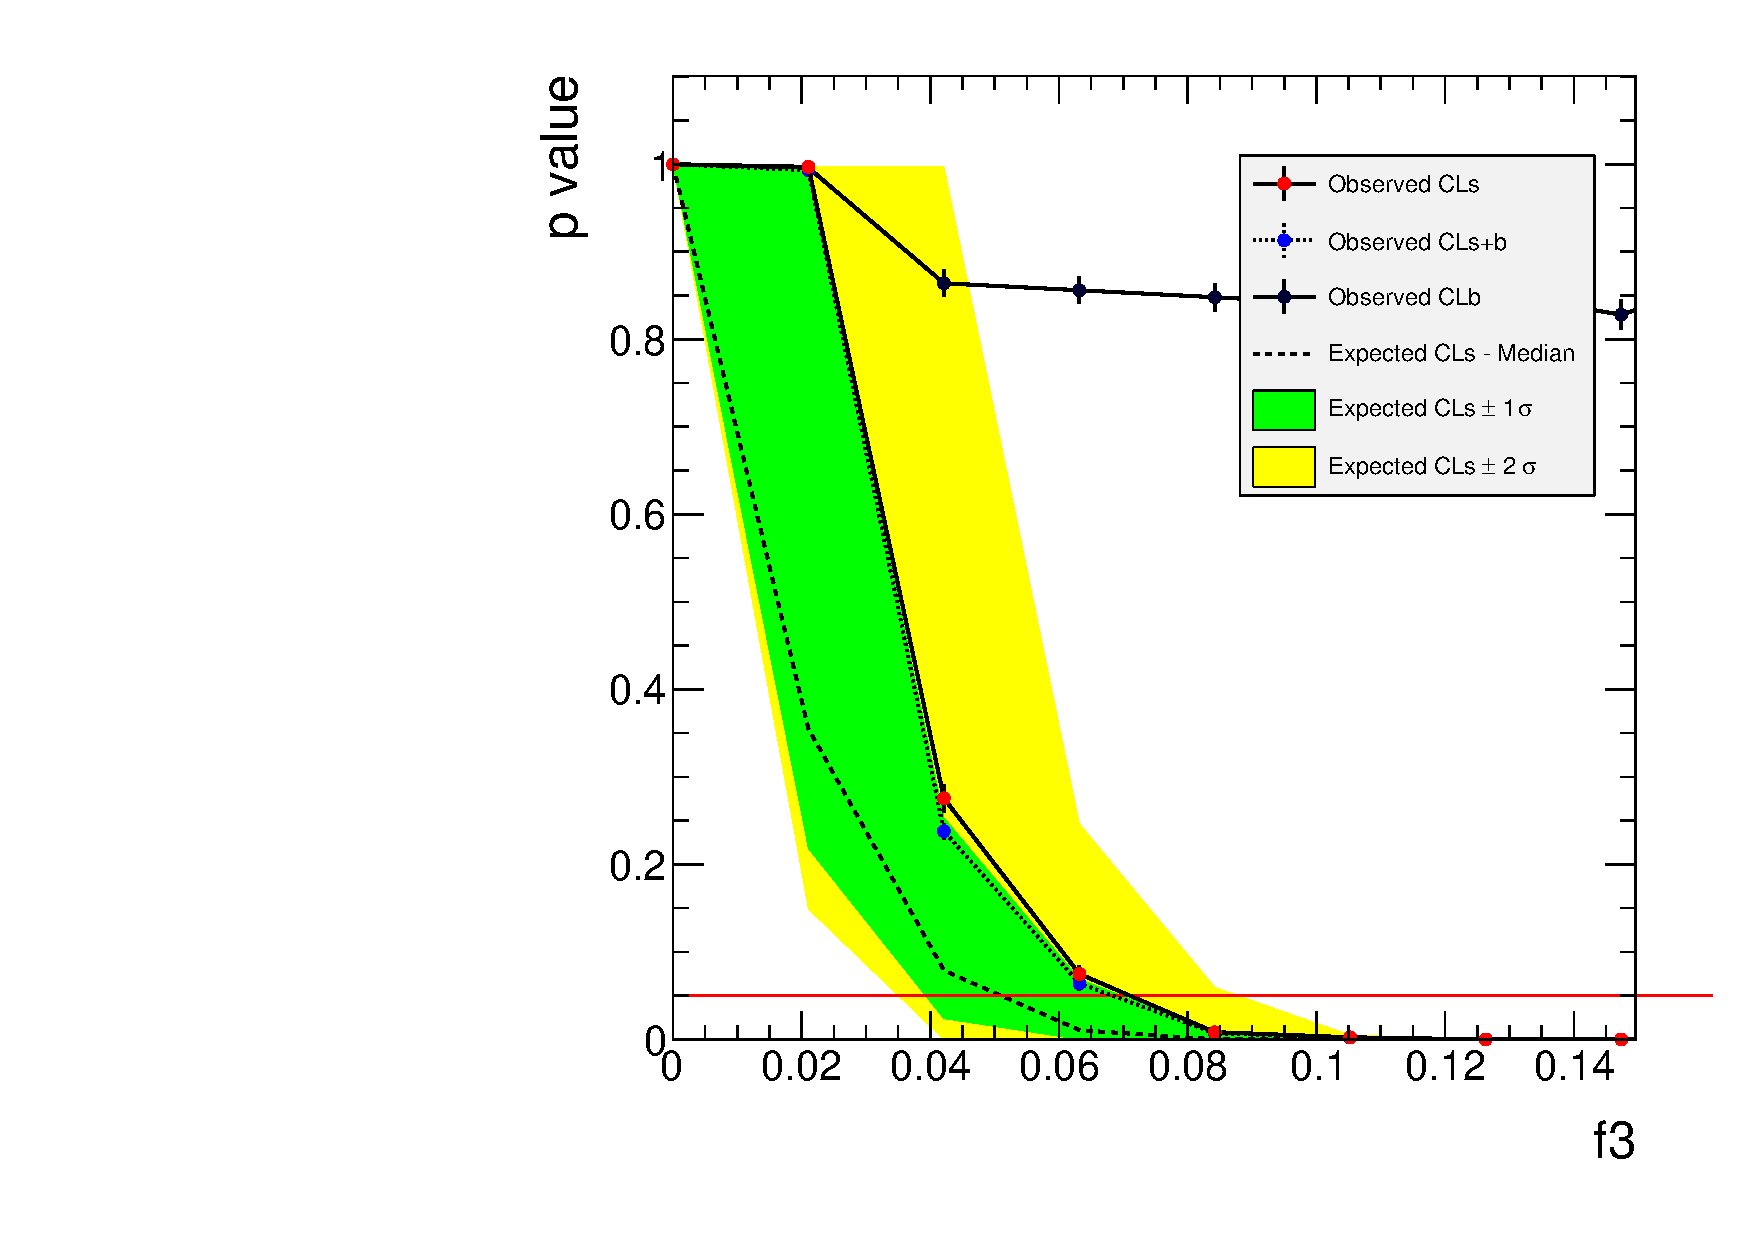
\includegraphics[angle=0,width=0.45\textwidth]{figures/limits/FC_0100}}
   \caption{Upper limit results for $R_3$ in \PbPb using the Feldman-Cousins method.
Shown is a $p$-value scan using 1000 pseudo experiments for each scanned point.  
The 95\% C.L. upper limit corresponds to the point where the observed CLs crosses the 0.05 horizontal/red line. 
%\emph{(Note: being updated)}
%Fig.~\ref{fig:FC_Centrality}: Upper limits vs number of participants using Feldman-Cousins.
}
    \label{fig:FC_results}
  \end{center}
\end{figure}



\subsubsection{Double ratio $\chi_{3}$ limits}

The same statistical instruments shown above are also used to set the limits for double ratio $\chi_{3}$.
Employing the Feldman Cousins technique, the upper limit at 95\% C.L. 
 is $\chi_{3} \leq 0.173 \pm 0.021$,  
as represented in \fig{fig:FCx3_0100}. 

\begin{figure}[hbtp]
  \begin{center}
    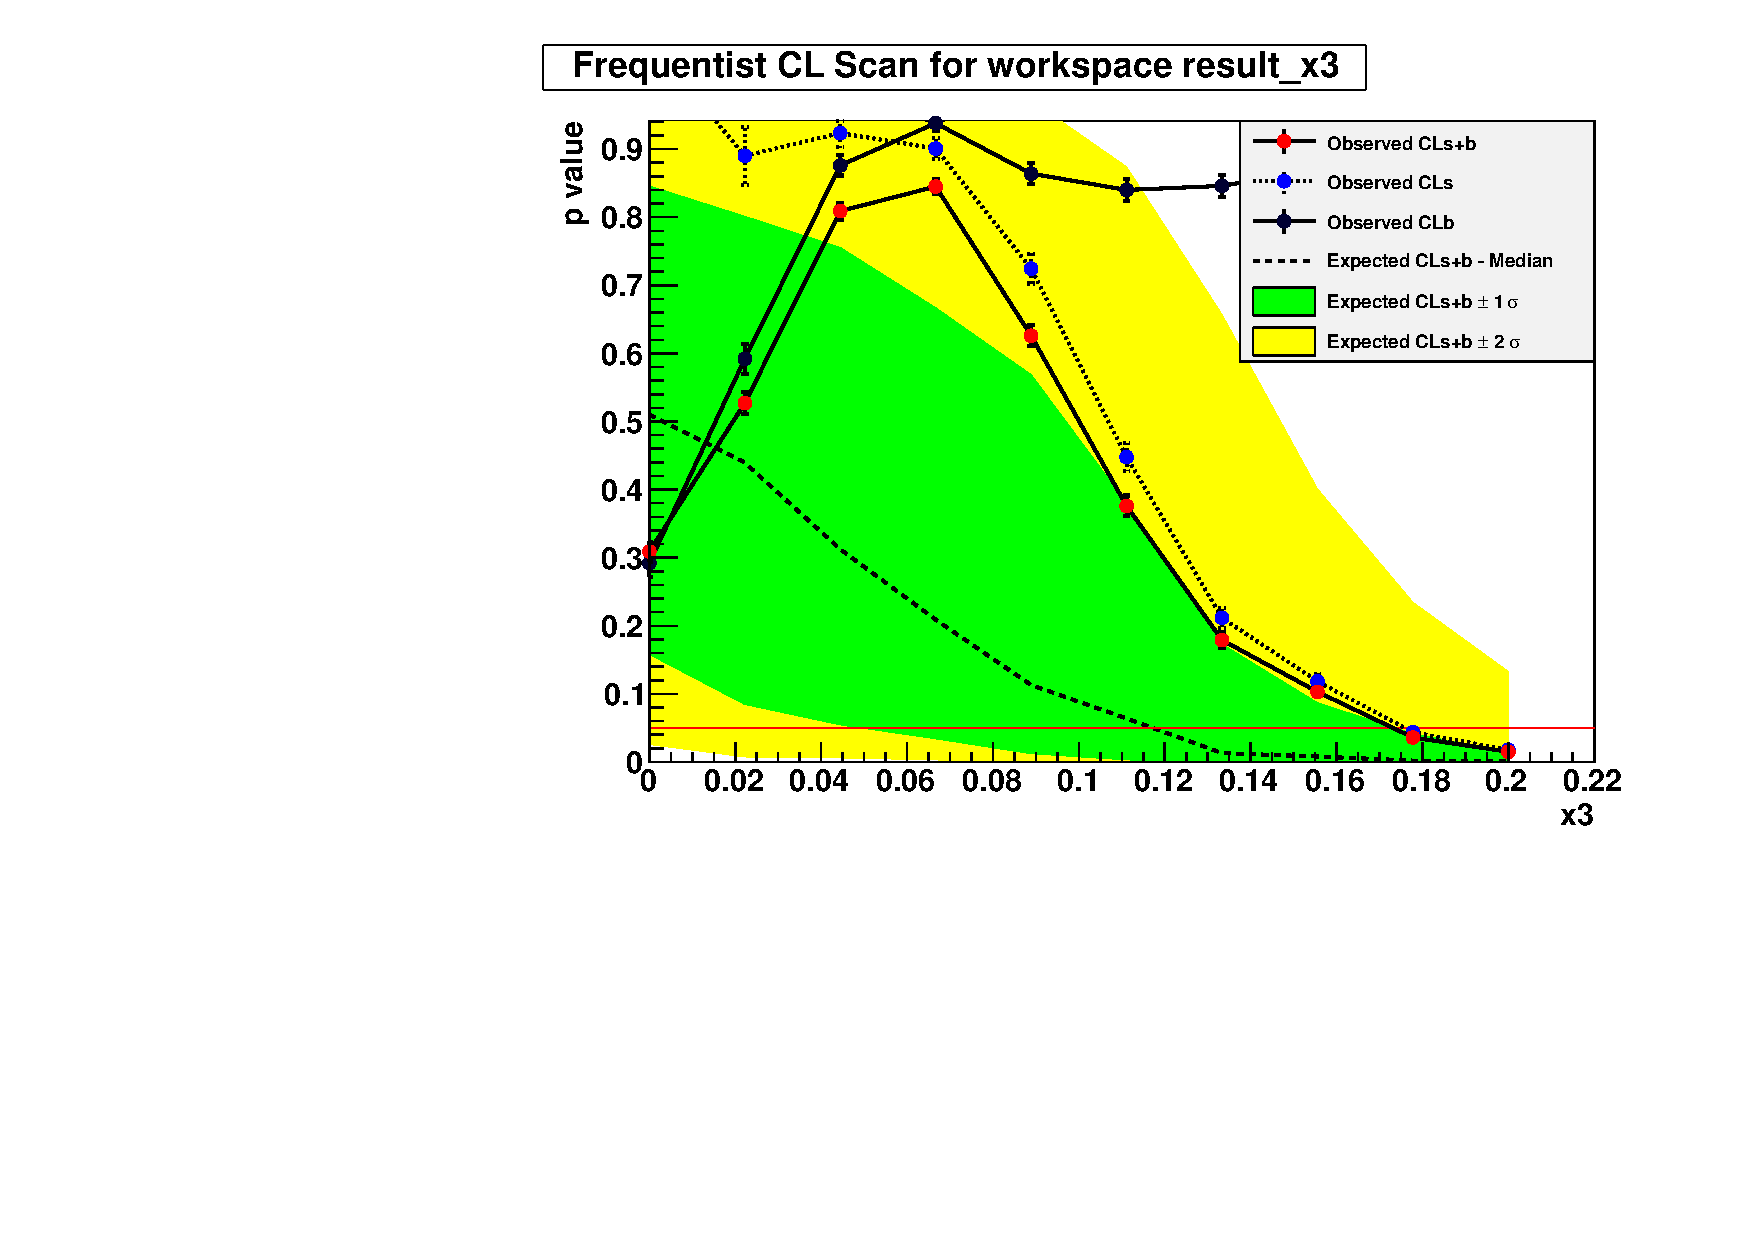
\includegraphics[angle=0,width=0.45\textwidth]{figures/limits/FC_chi3_0100.pdf}
    \caption{95\% interval on $\chi_{3}$ with Feldman Cousins technique after including systematic uncertainties. }
    \label{fig:FCx3_0100}
  \end{center}
\end{figure}


Using the profile likelihood calculator as cross-check, the 95\% C.L. interval is
$\chi_{3} \in   [0.042, 0.104]$, 
which is shown in figure \fig{fig:PLRx3_0100}.  
  

\begin{figure}[hbtp]
  \begin{center}
    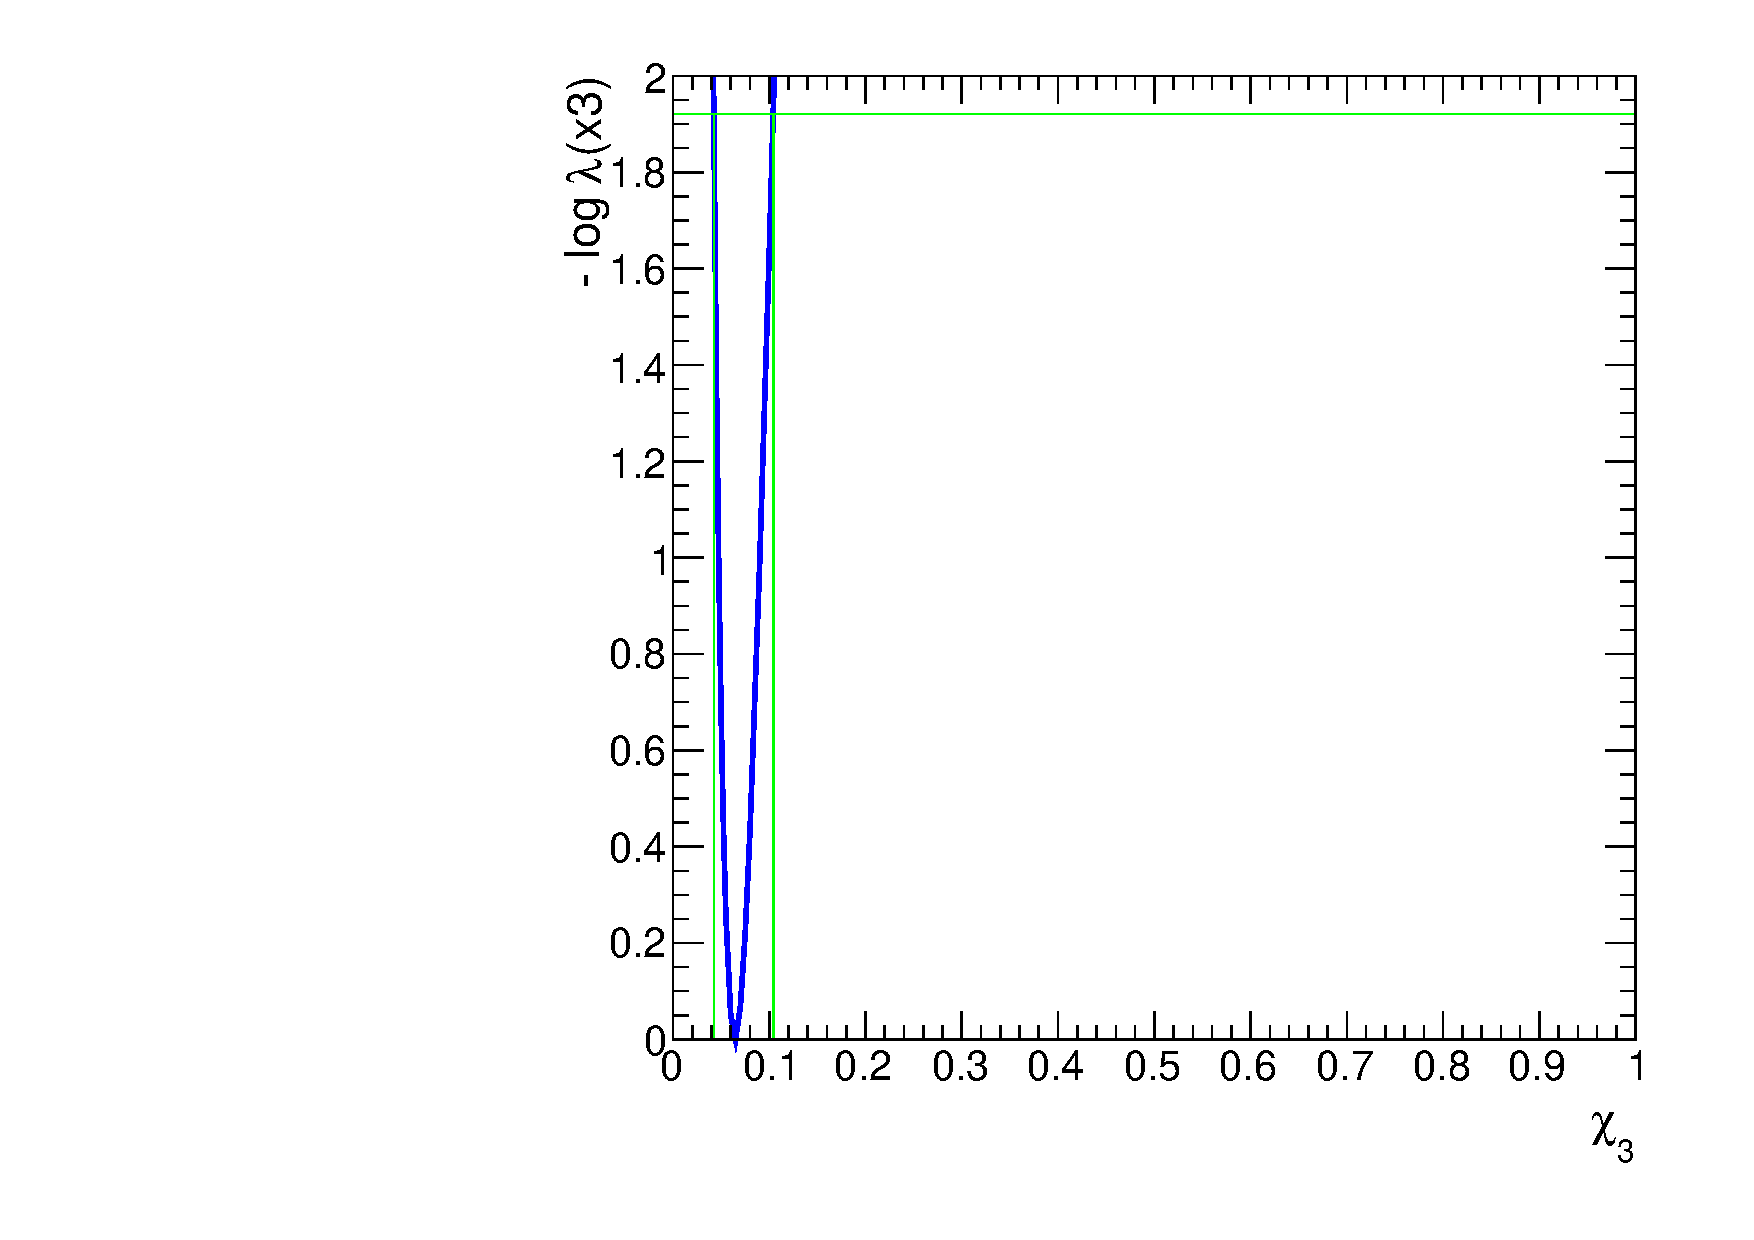
\includegraphics[angle=0,width=0.45\textwidth]{figures/limits/PLRx3_0100.pdf}
    \caption{95\% interval on $\chi_{3}$ with profile likelihood calculator not including systematic uncertainties. }
    \label{fig:PLRx3_0100}
  \end{center}
\end{figure}
